% !TEX TS-program = pdfLaTeX+shellescape
% !TEX encoding = UTF-8 Unicode

\documentclass{standalone}
\usepackage{pgfplots}
\pgfplotsset{compat=1.17}

\begin{document}
    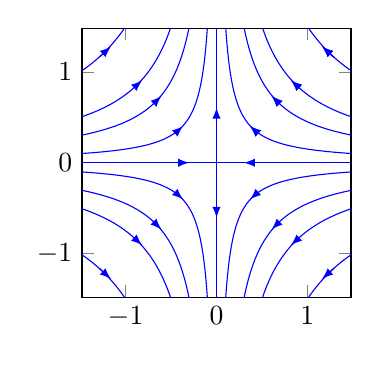
\begin{tikzpicture}[baseline]
        \begin{axis}[
            scale=0.6, % scale
            % view = {0}{90},
            xmin=-1.48,xmax=1.48,ymin=-1.48,ymax=1.48, % range of plot
            % legend style={at={(axis cs: 1,0)}, anchor=south east}, % position of legends
            % unit vector ratio = {1, 1, 1}, % aspect ratio
            unit vector ratio = {1, 1}, % aspect ratio
            % axis lines = box, % middle or box
            %axis x line = bottom, % top, middle, bottom, none: axis x line* = ... removes arrow heads
            %axis y line = left, % left, center, right, none: axis y line* = ... removes arrow heads
            %xlabel = {$x$}, ylabel = {$y$}, % axis labels 
        ]
            \addplot[blue, domain=0:1, samples=100]({1.5*exp(-x)}, {1.0*exp(x)});
            \addplot[blue, domain=0:2, samples=100]({1.5*exp(-x)}, {0.5*exp(x)});
            \addplot[blue, domain=0:2, samples=100]({1.5*exp(-x)}, {0.3*exp(x)});
            \addplot[blue, domain=0:3, samples=100]({1.5*exp(-x)}, {0.1*exp(x)});
            \addplot[blue, domain=0:10, samples=100]({1.5*exp(-x)}, {0.0*exp(x)});
            \addplot[blue, domain=0:1, samples=100]({-1.5*exp(-x)}, {1.0*exp(x)});
            \addplot[blue, domain=0:2, samples=100]({-1.5*exp(-x)}, {0.5*exp(x)});
            \addplot[blue, domain=0:2, samples=100]({-1.5*exp(-x)}, {0.3*exp(x)});
            \addplot[blue, domain=0:3, samples=100]({-1.5*exp(-x)}, {0.1*exp(x)});
            \addplot[blue, domain=0:10, samples=100]({-1.5*exp(-x)}, {0.0*exp(x)});
            \addplot[blue, domain=0:1, samples=100]({1.5*exp(-x)}, {-1.0*exp(x)});
            \addplot[blue, domain=0:2, samples=100]({1.5*exp(-x)}, {-0.5*exp(x)});
            \addplot[blue, domain=0:2, samples=100]({1.5*exp(-x)}, {-0.3*exp(x)});
            \addplot[blue, domain=0:3, samples=100]({1.5*exp(-x)}, {-0.1*exp(x)});
            \addplot[blue, domain=0:1, samples=100]({-1.5*exp(-x)}, {-1.0*exp(x)});
            \addplot[blue, domain=0:2, samples=100]({-1.5*exp(-x)}, {-0.5*exp(x)});
            \addplot[blue, domain=0:2, samples=100]({-1.5*exp(-x)}, {-0.3*exp(x)});
            \addplot[blue, domain=0:3, samples=100]({-1.5*exp(-x)}, {-0.1*exp(x)});
            \addplot[blue, domain=0:10, samples=100]({0.0*exp(-x)}, {1.5*exp(-x)});
            \addplot[blue, domain=0:10, samples=100]({0.0*exp(-x)}, {-1.5*exp(-x)});
            \addplot[blue, variable=\t, samples=2, domain=-0.5:0.15, -latex, quiver={u={-1.5*exp(-t)}, v={1.0*exp(t)}, scale arrows=0.1}]({1.5*exp(-t)}, {1.0*exp(t)});
            \addplot[blue, variable=\t, samples=2, domain=-0.5:0.5, -latex, quiver={u={-1.5*exp(-t)}, v={0.5*exp(t)}, scale arrows=0.1}]({1.5*exp(-t)}, {0.5*exp(t)});
            \addplot[blue, variable=\t, samples=2, domain=-1:0.8, -latex, quiver={u={-1.5*exp(-t)}, v={0.3*exp(t)}, scale arrows=0.1}]({1.5*exp(-t)}, {0.3*exp(t)});
            \addplot[blue, variable=\t, samples=2, domain=-1:1.3, -latex, quiver={u={-1.5*exp(-t)}, v={0.1*exp(t)}, scale arrows=0.1}]({1.5*exp(-t)}, {0.1*exp(t)});
            \addplot[blue, variable=\t, samples=2, domain=-1:1.5, -latex, quiver={u={-1.5*exp(-t)}, v={0.0*exp(t)}, scale arrows=0.1}]({1.5*exp(-t)}, {0.0*exp(t)});
            \addplot[blue, variable=\t, samples=2, domain=-0.5:0.15, -latex, quiver={u={1.5*exp(-t)}, v={1.0*exp(t)}, scale arrows=0.1}]({-1.5*exp(-t)}, {1.0*exp(t)});
            \addplot[blue, variable=\t, samples=2, domain=-0.5:0.5, -latex, quiver={u={1.5*exp(-t)}, v={0.5*exp(t)}, scale arrows=0.1}]({-1.5*exp(-t)}, {0.5*exp(t)});
            \addplot[blue, variable=\t, samples=2, domain=-1:0.8, -latex, quiver={u={1.5*exp(-t)}, v={0.3*exp(t)}, scale arrows=0.1}]({-1.5*exp(-t)}, {0.3*exp(t)});
            \addplot[blue, variable=\t, samples=2, domain=-1:1.3, -latex, quiver={u={1.5*exp(-t)}, v={0.1*exp(t)}, scale arrows=0.1}]({-1.5*exp(-t)}, {0.1*exp(t)});
            \addplot[blue, variable=\t, samples=2, domain=-1:1.5, -latex, quiver={u={1.5*exp(-t)}, v={0.0*exp(t)}, scale arrows=0.1}]({-1.5*exp(-t)}, {0.0*exp(t)});
            \addplot[blue, variable=\t, samples=2, domain=-0.5:0.15, -latex, quiver={u={1.5*exp(-t)}, v={-1.0*exp(t)}, scale arrows=0.1}]({-1.5*exp(-t)}, {-1.0*exp(t)});
            \addplot[blue, variable=\t, samples=2, domain=-0.5:0.5, -latex, quiver={u={1.5*exp(-t)}, v={-0.5*exp(t)}, scale arrows=0.1}]({-1.5*exp(-t)}, {-0.5*exp(t)});
            \addplot[blue, variable=\t, samples=2, domain=-1:0.8, -latex, quiver={u={1.5*exp(-t)}, v={-0.3*exp(t)}, scale arrows=0.1}]({-1.5*exp(-t)}, {-0.3*exp(t)});
            \addplot[blue, variable=\t, samples=2, domain=-1:1.3, -latex, quiver={u={1.5*exp(-t)}, v={-0.1*exp(t)}, scale arrows=0.1}]({-1.5*exp(-t)}, {-0.1*exp(t)});
            \addplot[blue, variable=\t, samples=2, domain=-0.5:0.15, -latex, quiver={u={-1.5*exp(-t)}, v={-1.0*exp(t)}, scale arrows=0.1}]({1.5*exp(-t)}, {-1.0*exp(t)});
            \addplot[blue, variable=\t, samples=2, domain=-0.5:0.5, -latex, quiver={u={-1.5*exp(-t)}, v={-0.5*exp(t)}, scale arrows=0.1}]({1.5*exp(-t)}, {-0.5*exp(t)});
            \addplot[blue, variable=\t, samples=2, domain=-1:0.8, -latex, quiver={u={-1.5*exp(-t)}, v={-0.3*exp(t)}, scale arrows=0.1}]({1.5*exp(-t)}, {-0.3*exp(t)});
            \addplot[blue, variable=\t, samples=2, domain=-1:1.3, -latex, quiver={u={-1.5*exp(-t)}, v={-0.1*exp(t)}, scale arrows=0.1}]({1.5*exp(-t)}, {-0.1*exp(t)});
            \addplot[blue, variable=\t, samples=2, domain=-0.5:0.15, -latex, quiver={u={-1.5*exp(-t)}, v={1.0*exp(t)}, scale arrows=0.1}]({1.5*exp(-t)}, {1.0*exp(t)});
            \addplot[blue, variable=\t, samples=2, domain=-0.5:0.5, -latex, quiver={u={-1.5*exp(-t)}, v={0.5*exp(t)}, scale arrows=0.1}]({1.5*exp(-t)}, {0.5*exp(t)});
            \addplot[blue, variable=\t, samples=2, domain=-1:0.8, -latex, quiver={u={-1.5*exp(-t)}, v={0.3*exp(t)}, scale arrows=0.1}]({1.5*exp(-t)}, {0.3*exp(t)});
            \addplot[blue, variable=\t, samples=2, domain=-1:1.3, -latex, quiver={u={-1.5*exp(-t)}, v={0.1*exp(t)}, scale arrows=0.1}]({1.5*exp(-t)}, {0.1*exp(t)});
            \addplot[blue, variable=\t, samples=2, domain=-1:1.0, -latex, quiver={u={0.0*exp(-t)}, v={-1.5*exp(-t)}, scale arrows=0.1}]({0.0*exp(-t)}, {-1.5*exp(-t)});
            \addplot[blue, variable=\t, samples=2, domain=-1:1.0, -latex, quiver={u={0.0*exp(-t)}, v={1.5*exp(-t)}, scale arrows=0.1}]({0.0*exp(-t)}, {1.5*exp(-t)});
        \end{axis}
    \end{tikzpicture}
\end{document}